\documentclass{article}
\usepackage[T1]{fontenc}
\usepackage{lmodern}
\usepackage{graphicx}
\usepackage{amsmath,amssymb}
\usepackage[a4paper,margin=2cm]{geometry}
\usepackage[absolute,overlay]{textpos}
\setlength{\TPHorizModule}{1mm}
\setlength{\TPVertModule}{1mm}
\usepackage[indonesian]{babel}
\usepackage{hyperref}
\setlength{\emergencystretch}{2em}
% unit: Halaman 21

\begin{document}

% === Halaman 21 (llm) ===

\vspace{196.02mm}

\begin{itemize}
    \item Hasil ekspansi, yaitu $E(R_{i-1})$ di-XOR-kan dengan $K_i$ menghasilkan blok A berukuran 48-bit:
    \[ E(R_{i-1}) \oplus K_i = A \]
    \vspace{50mm}
    \item Blok $A$ dikelompokkan menjadi 8 kelompok, masing-masing 6 bit, dan menjadi masukan bagi proses substitusi.
    \item Ada 8 matriks substitusi, masing-masing dinyatakan dengan kotak-S.
    \item Kotak-S menerima masukan 6 bit dan memberikan luaran 4 bit.
\end{itemize}

% deskripsi: Diagram alir proses enkripsi yang menunjukkan tahap ekspansi dari R_{i-1} (32 bit) menjadi 48 bit, operasi XOR dengan K_i untuk menghasilkan blok A, proses substitusi melalui kotak-S (S1 sampai S8), dan tahap permutasi P(B).
% bbox normalisasi: [0.5100, 0.2500, 0.9600, 0.9100]
\begin{textblock*}{94.50mm}(107.10mm,74.25mm)
\noindent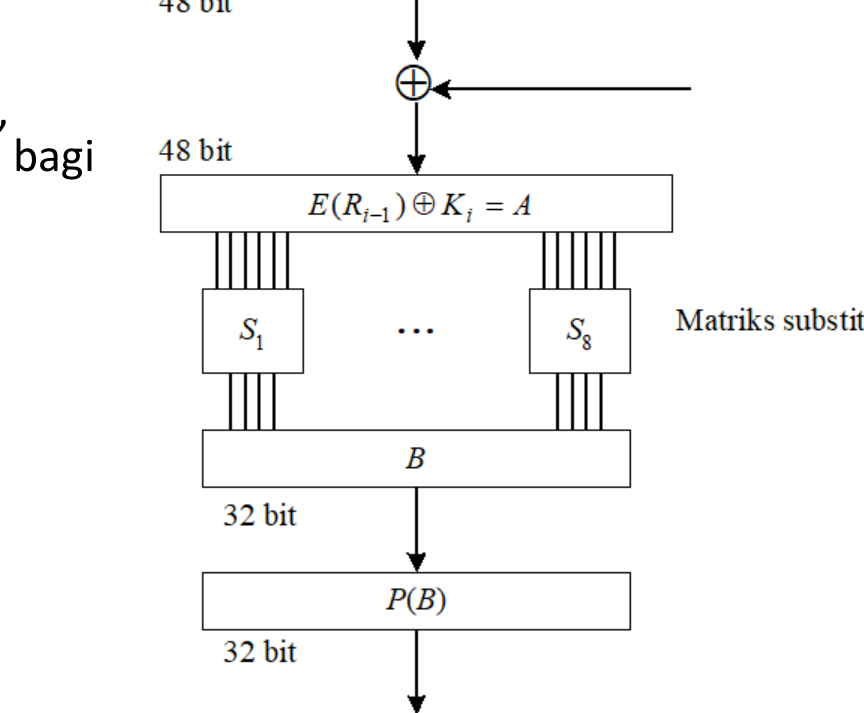
\includegraphics[width=94.50mm,height=196.02mm]{../../images/llm/page_021_img_01.png}%
\end{textblock*}

\end{document}
